\section{\mc 分類手法}
分類問題の説明を行う。

\subsection{\rm Linear Discriminant Analysis(LDA)}
\label{subsec:LDA}
Linear Discriminant Analysis(LDA)は統計分析において伝統的に用いられてきた歴史ある手法である。
LDAでは多次元データを部分空間で切り取り、切り取った空間で分類超平面を構築することでクラス分類を行う。
分類超平面を構築する手段を与えなければ、LDAは特徴量抽出手法としても機能する。
まず、多次元データ\(x\in \mathbb R^D\)を基底\(w \in \mathbb R^D\)へ射影すると、
以下の式で表されるスカラー値を獲得できる。
\begin{equation}
    z = w^Tx \in \mathbb R
\end{equation}
zに対してある閾値を設定し、\(z \geq -w_0\)の場合はクラス\(C_1\)とし、そうでない場合は
クラス\(C_2\)であるとすることで分類器を獲得できる。
多次元データを1次元空間へ射影した場合には多くの情報損失が生ずるが、
\(w\)の取り方を上手く調整することによって、クラス分類を行いやすい射影を選択できる。
まず以下のようにクラス毎の平均ベクトル\(m_1,m_2\)を定義する。
\begin{eqnarray}
    m_{1} & = & \frac{1}{|C_1|}\sum_{x\in C_1}x  \\
    m_{2} & = & \frac{1}{|C_2|}\sum_{x\in C_2}x
\end{eqnarray}
ここに、\(|C_i|\)はクラス\(C_i\)に属するデータの数である。
クラス\(C_1\)とクラス\(C_2\)の平均間の距離が射影先で大きな値となれば、
異なるクラスのデータは平均的に離れて配置され、クラス分類を行いやすい射影になっていると想定できる。
従って、まずは以下の距離の最大化を考慮する。
\begin{equation}
    d=|w^T(m_1-m_2)|
    \label{eq:dis}
\end{equation}
しかし実際には(\ref{eq:dis})の最大化を考慮しただけでは分類が上手く行くとは限らない(図\ref{fig:mean_dis})。
射影先での各クラスのデータの分散が大きい場合には、異なるクラスのデータが重なってしまう場合が生じるからである。
\begin{figure}
    \centering
    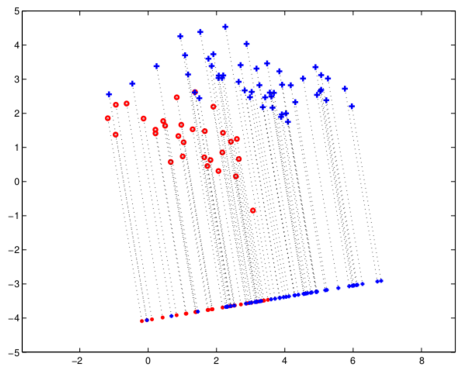
\includegraphics[width=12cm]{images/mean_dis.png}
    \caption{クラス毎の平均間の距離を射影先で最大化した判別分析}
    \label{fig:mean_dis}
\end{figure}
この問題を解決するためにはデータの分散を考慮する必要がある。
まず射影先での各クラスの分散は以下で表記できる。
\begin{eqnarray}
    \sigma^2_{1} & = & \sum_{x\in C_1}\{w^T(x-m_1)\}^2  \\
    \sigma^2_{2} & = & \sum_{x\in C_2}\{w^T(x-m_2)\}^2
\end{eqnarray}
ここで、全データのクラス毎の分散の和を総クラス内分散として以下で定義する。
\begin{equation}
    \sigma^2  = \sigma^2_1 + \sigma^2_2
    \label{eq:sig}
\end{equation}
総クラス内分散(\ref{eq:sig})を小さくしながらクラス間の平均の距離(\ref{eq:dis})を大きくすることを考慮し
LDAでは以下の評価関数を用いる。
\begin{eqnarray}
    J(w) & = & \frac{d^2}{\sigma^2} \nonumber \\
    & = & \frac{\{w^T(m_1-m_2)\}^2}{\sum_{x\in C_1}\{w^T(x-m_1)\}^2 + \sum_{x\in C_2}\{w^T(x-m_2)\}^2}
    \label{eq:lda_obj}
\end{eqnarray}
このクラス間の平均とクラス内の分散を考慮した評価関数を用いることで、
射影先でデータがクラス毎に小さくまとまり、かつ異なるクラスのデータがなるべく離れるようになる(図\ref{fig:var_dis})。
\begin{figure}
    \centering
    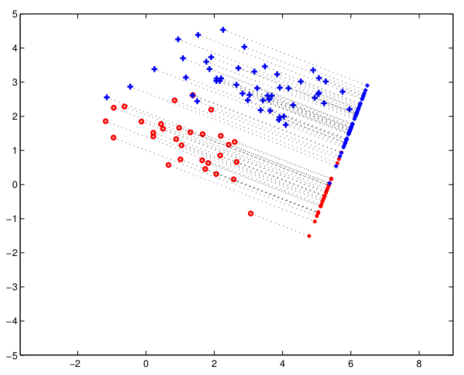
\includegraphics[width=12cm]{images/var_dis.png}
    \caption{クラス毎の平均間の距離を射影先で最大化し、総クラス内分散を最小化した判別分析}
    \label{fig:var_dis}
\end{figure}

1次元の空間(数直線上)でクラス毎にデータが上手く分離できた後、
数直線上に閾値\(w_0=(m_1+m_2)/2\)を設けることで分離平面が得られる。
これはクラス毎の平均値の平均値によって分離平面を設定したことに相当する。
しかし、射影のされ方によってはこの閾値は適当ではない。
より精密な分類を行うためには、\(z=w^Tx\)がクラス毎に異なるガウス分布から生じる確率変数だと考え、
クラス\(C_i\)の条件付き確率\(p(z|C_i)\)を算出した判別基準を設け、条件付き確率が大きいクラスへ分類するなどの方法を取る。
% ガウス分布を仮定した場合における判別基準は、マハラノビス距離が近いクラスへ分類することと等価である。
% 必ずしもガウス分布であるという仮定は必要ないが、\(z\)は複数の確率変数の線型結合であるため
% 中心極限定理によりこの仮定は正当化されうる。

またLDAの評価関数(\ref{eq:lda_obj})は以下のように変形が可能である。
\begin{eqnarray}
    \label{eq:lda_obj_mat}
    J(w) 
    & = & \frac{\{w^T(m_1-m_2)\}^2}{\sum_{x\in C_1}\{w^T(x-m_1)\}^2 + \sum_{x\in C_2}\{w^T(x-m_2)\}^2} \nonumber \\
    & = & \frac{w^T(m_1-m_2)(m_1-m_2)^Tw} {w^T\left\{ \sum_{x\in C_1} (x-m_1)(x-m_1)^T + \sum_{x\in C_2} (x-m_2)(x-m_2)^T \right\}w} \nonumber \\
    & = & \frac{w^TS_Bw} {w^TS_Ww} \\
    \nonumber 
    % & where & \nonumber \\ 
    % & &S_B = (m_1-m_2)(m_1-m_2)^T \\
    % & &S_W = \sum_{x\in C_1} (x-m_1)(x-m_1)^T + \sum_{x\in C_2} (x-m_2)(x-m_2)^T
\end{eqnarray}
ここで
\begin{eqnarray}
    S_B &=& (m_1-m_2)(m_1-m_2)^T \\
    S_W &=& \sum_{x\in C_1} (x-m_1)(x-m_1)^T + \sum_{x\in C_2} (x-m_2)(x-m_2)^T
\end{eqnarray}
である。このとき\(S_B\)をクラス間共分散行列、\(S_W\)をクラス内共分散行列と言う。
(\ref{eq:lda_obj_mat})を\(w\)に関して微分して\(0\)と置くことで問題は解析的に解くことができる。
また問題は一般化固有値問題となり、複数の固有ベクトルを用いて多次元の特徴量を獲得することも可能である。

\subsection{\rm Support Vector Machine(SVM)}
脳波の分類ではSupport Vector Machine(SVM)の応用例もある。
基本的にSVMはマージン最大化の考えによって汎化性能の向上に成功した
2クラス分類のための線形分類器である。まずマージン最大化という概念について説明する。
マージンとは端的に述べるとデータ点と分類超平面との距離のことを表す。
学習データに対してマージンを最大化することで、学習データが空間上で僅かに移動した際にも
誤分類を起こしづらくなると期待できる。
SVMではこのマージン最大化によって以下の分類超平面を定める。
\begin{equation}
    y(x) = w^Tx + w_0
    \label{eq:displane}
\end{equation}
ここに\(x\)は\(D\)次元のデータベクトルであり、\(w\)は\(D\)次元のパラメータベクトルである。
\(w_0\)もスカラーパラメータであり閾値の役割を担う。
分類面の役割により\(y(x)\)は\(x\)がクラス\(C_1\)に属する場合には正の値を、\(C_2\)に属する場合には負の値を取るように学習される。
ここで、(\ref{eq:displane})の超平面と、あるデータ点\(x_n\)との距離は以下で表される。
\begin{equation}
    |r| = \frac{|y(x_n)|}{|w|}
    \label{eq:distance}
\end{equation}
ここで、\(x_n\)がクラス\(C_1\)に属する場合は\(t_n=1\)とし、クラス\(C_2\)に属する場合には
\(t_n=-1\)と定めた\(t_n\)を導入する。
さらに\(x_n\)には分類面から最も近いデータ点のみを考慮することとし、
そのときの\(|r|\)をマージンと呼び以下で表す。
\begin{equation}
    |r|_{margin} = \min_{x_n}\frac{t_ny(x_n)}{|w|}
    \label{eq:margin}
\end{equation}
この(\ref{eq:margin})を最大化するようにパラメータを決定することで
マージン最大化を実現することができる。
従って、SVMのパラメータ決定は以下の最適化問題によって定式化される。
\begin{equation}
    \argmax_{w_0,w}\left(\min_{x_n}\frac{t_ny(x_n)}{|w|}\right)
    \label{eq:obj margin}
\end{equation}
しかしこの最適化問題において、\(w,w_0\)の大きさは本質的ではない。
なぜなら\(w,w_0\)を同時に\(kw,kw_0\)と定数倍した場合にも(\ref{eq:margin})の値は変化しないためである。
従って、\(w,w_0\)の大きさに関して制約を設ける必要がある。
そこで分類面から最も近い\(x_n\)に関して\(t_n(w^Tx+w_0)=1\)
となるような制約を\(w,w_0\)に対して要請する。
この条件式に伴って、任意のデータ点において\(t_n(w^Tx+w_0) \geq 1 \)という制約が与えられる。
最終的にマージン最大化問題(\ref{eq:obj margin})は以下で定式化される。
\begin{equation}
    \begin{aligned}
    & \argmin_{w_0,w}
    & & \frac{|w|^2}{2}  \\
    & \text{s.t.}
    & &  t_n(w^Tx+w_0)  \geq 1 
    \end{aligned}
    \label{eq:obj nonlinear}
\end{equation}
目的関数の分母は、単に勾配を計算する際に約分できるというテクニックによるものである。
分子の二乗は、最適化問題の解を変更せずに勾配計算などを容易に行うための変形である。
図\ref{fig:margin}に分類面の定め方によりマージンが異なっている様子を見ることができる。
左右いずれの図も学習データに対して正しく分類が行える分類面になっているが、
新規のデータに対しての分類結果が異なってくる。SVMでは右図の分類面の方が優れていると考える場合に用いる手法である。
\begin{figure}
    \centering
    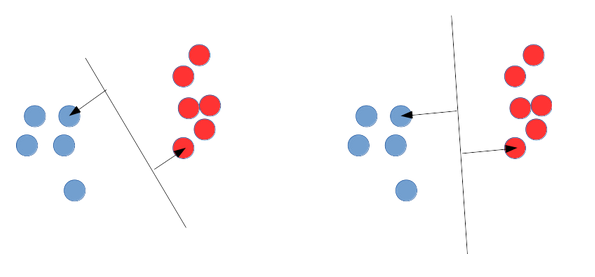
\includegraphics[width=12cm]{images/margin.png}
    \caption{分類面によってマージンの大きさが異なる様子}
    \label{fig:margin}
\end{figure}
ここまで線形分類を行う場合のSVMを見てきたが、
一般的に線形分類器はデータ点を非線形関数\(\phi(\cdot)\)によって別の特徴空間へ写像し、
特徴空間上で線形分類を行う問題へ拡張することができる。SVMでは分類超平面を以下の式によって構築することに相当する。
\begin{equation}
    y(x) = w^T \phi (x) + w_0
    \label{eq:displane2}
\end{equation}
この場合においてもこれまでと同様の議論で最適化問題を以下のように定式化できる。
\begin{equation}
    \begin{aligned}
    & \argmin_{w_0,w}
    & & \frac{|w|^2}{2} \\
    & \text{s.t.}
    & &  t_n(w^T\phi(x)+w_0)  \geq 1 
    \end{aligned}
    \label{eq:obj nonlinear}
\end{equation}

実データは線形分離不可能な場合が多いため、
通常SVMを用いる場合は上記のような非線形に拡張されたものを用いる。
また実データは異なるクラスのデータが重なって分布することも多々あるため、
厳密な分類を行うことは不可能な場合が多い。
そういった場合に対応したソフトマージンと呼ばれる考えがあり、
学習データの誤分類に対して寛容になる指標を導入する。
このソフトマージンの考え方は機械学習で過学習抑制に用いられる正則化の考えと本質的には変わりない。
また、制約付き最適化問題をラグランジュ法によって変形することで双対問題を獲得することができる。
双対問題においては非線形変換後の空間での内積のみが必要となり、
具体的な非線形変換の計算をデータ\(x\)に対して実施する必要はない。
すなわち、非線形変換\(\phi(x)\)による特徴空間への写像を具体的に考える代わりに、
最終的に計算の必要性がある内積\(\phi(x)^T\phi(x')\)を定義することでSVMの非線形への拡張が可能である。
このような方法はカーネル法として知られており、このときに用いられる内積計算をカーネル
\(k(x,x')=\phi(x)^T\phi(x')\)と呼ぶ。カーネルを定めることが特徴空間の設計を行うことに相当するが、
BCIも含めた多くの応用では既に知られた優れた性質を持つカーネルを活用することがほとんどである。
以下に代表的なカーネルについて記載する。
\begin{description}
    \item[・線形カーネル:非線形変換を行わないことに対応。] \mbox{}
    \begin{center} \(k(x,x')=x^Tx'\) \end{center}
    \item[・多項式カーネル:多項式関数による非線形変換に対応。] \mbox{} 
    \begin{center} \(k(x,x')=(x^Tx' + c)^M\) \end{center}
    \item[・ガウス基底カーネル:特徴空間が無限次元となる。] \mbox{}\par
    \begin{center} \(k(x,x')=\exp\left(-\frac{|x-x'|^2}{2\sigma^2}\right)\) \end{center}
\end{description}
通常、カーネルを用いる場合にはハイパーパラメータが付随する。多項式カーネルの場合はスカラーの\(c,M\)、
ガウス基底カーネルの場合はスカラーの\(\sigma\)がハイパーパラメータとなり、これらの調整次第で
得られる分類面は異なる。
応用上はソフトマージンカーネルSVMを用いればよく、ソフトマージンのハイパーパラメータとカーネルの設計を変えることで
通常の線形SVMの働きをさせることも可能である。
図\ref{fig:linear}-\ref{fig:kernel}に2次元データに対するSVMの分類境界を示す。
図\ref{fig:xor}の通り、線形SVMでは線形分離不可能な問題に対して不適切な境界を設ける。
\begin{figure}[t]
    \begin{minipage}{0.5\hsize}
     \begin{center}
      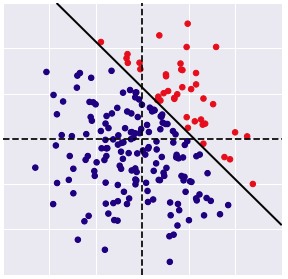
\includegraphics[width=50mm]{images/linearSVM.png}
     \end{center}
     \caption{線形SVM(線形分離可能)}
     \label{fig:linear}
    \end{minipage}
    \begin{minipage}{0.5\hsize}
     \begin{center}
      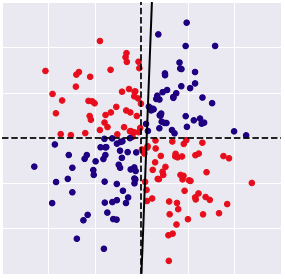
\includegraphics[width=50mm]{images/xorlinearSVM.png}
     \end{center}
     \caption{線形SVM(線形分離不可能)}
     \label{fig:xor}
    \end{minipage}
\end{figure}
\begin{figure}[t]
    \centering
    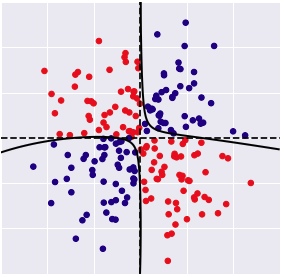
\includegraphics[width=70mm]{images/xorkernelSVM.png}
    \caption{ガウシアンカーネルSVM(線形分離不可能)}
    \label{fig:kernel}
\end{figure}

ソフトマージンカーネルSVMの識別関数は以下で表される。
\begin{equation}
    y(x) = \sum_{n=1}^Na_nt_nk(x,x_n) + b
    \label{dis_kernel}
\end{equation}
ここで学習データの数を\(N\)としている。
また\(a_n\)はスカラーのパラメータであり、ラグランジュ法で双対問題を考えた際のラグランジュ乗数である。
また最適化問題は以下で定式化される。
\begin{equation}
    \begin{aligned}
    & \argmax_{a_1,\cdots,a_N}
    & & \sum_{n=1}^N a_n - \frac{1}{2}\sum_{i=1}^N \sum_{j=1}^N a_ia_jt_it_jk(x_i,x_j) \\
    & \text{s.t.}
    & & 0 \leq a_n \leq C  \\
    & & &  \sum_{n=1}^N a_nt_n=0
    \end{aligned}
    \label{eq:kernel SVM}
\end{equation}
ここに\(C\)はソフトマージンのハイパーパラメータでありスカラーである。値が小さいほど\(a_n\)の取れる範囲が制限され、値が大きいほど誤分類に寛容となる。
最適化問題の解である\(a_1,\cdots,a_N\)と任意の\(n\)を選んで以下の条件式に代入することで閾値\(b\)も求まる。

\begin{equation}
    t_n\left( \sum_{m=1}^Na_mt_mk(x_n,x_m) + b \right)=1
    \label{eq:bias}
\end{equation}
ただし、(\ref{eq:bias})は無駄な計算も含まれている。\(a_n=0\)となるような\(x_n\)に対して
\(\sum_{n=1}^Na_nt_nk(x,x_n)\)の計算を実行する必要はない。
\(a_n\neq0\)となっている\(x_n\)のことをサポートベクトルと呼び、
実際にはサポートベクトルのみ計算に考慮すれば良い。
このことは新規のデータに対して(\ref{dis_kernel})の計算を行うときも同様である。
従って学習後に保持しておかねければならないデータはサポートベクトルのみに限定でき、
実用上省メモリに貢献できる。

\subsection{\rm Logistic Regression(LR)}
Logistic Regression(LR)は対数オッズ比を線形モデルで表現した分類手法である。
クラス分類においてデータ\(x\)がクラス\(C_i\)に属する確率を\(p(y=C_i\mid x)\)と表す。
この時、事象\(y=C_i\)のオッズ比は以下で表される。
\begin{equation}
    odds(y=C_i) = \frac{p(y=C_i \mid x)}{1-p(y=C_i \mid x)}
    \label{eq:odds}
\end{equation}
2クラス分類においては\(odds(y=C_1) \geq 1\)であれば\(C_1\)に分類する
などの規則を設けることで分類が可能になる。
ここで、対数オッズは以下で表される。
\begin{equation}
    logodds(y=C_i) = \log \left\{ \frac{p(y=C_i \mid x)}{1-p(y=C_i \mid x)} \right\}
    \label{eq:logodds}
\end{equation}
(\ref{eq:odds})が\(1\)以上の値となる時、(\ref{eq:logodds})は\(0\)以上の値となる。
LRでは多次元データ\(x\in \mathbb R^D\)に対して\(w \in \mathbb R^D\)として、
線形モデル\(z=w^Tx \in \mathbb R\)によって対数オッズ比を出力するモデルを構築する。
\(y = C_1\)の対数オッズ比を線形モデルで表現すると以下で表される。
\begin{equation}
    \log \left\{ \frac{p(y=C_1 \mid x)}{1-p(y=C_1 \mid x)} \right\} = w^Tx
    \label{eq:logoddsmodel}
\end{equation}
この時、以下の式変形によってよく知られたシグモイド関数\(\sigma(z)=1/(1+\exp(-z))\)が導出される。
\begin{eqnarray}
    && \log \left\{ \frac{p(y=C_1 \mid x)}{1-p(y=C_1 \mid x)} \right\}  =  w^Tx \nonumber \\
    \iff && \frac{p(y=C_1 \mid x)}{1-p(y=C_1 \mid x)}  =  \exp(w^Tx) \nonumber \\
    \iff && \frac{1}{p(y=C_1 \mid x)}-1  =  \exp(-w^Tx) \nonumber \\
    \iff && p(y=C_1 \mid x)  =  \frac{1}{1+\exp(-w^Tx)} 
    \label{eq:logisticmodel}
\end{eqnarray}
シグモイド関数に関しては、
\begin{eqnarray}
    \label{eq:logminas}
    \sigma(-z) = 1-\sigma(x) \\
    \sigma'(z) = \sigma(z)(1-\sigma(z))
\end{eqnarray}
という性質が知られている。
ここで\(y=C_1\)という事象を\(y=1\)に対応させ、\(y=C_2\)という事象を\(y=-1\)に対応させると、
(\ref{eq:logisticmodel})と(\ref{eq:logminas})用いて、
\begin{equation}
    p(y\mid x,w) = \sigma(yw^Tx)
\end{equation}
とすることができる。{\rm i.i.d.}を仮定して対数尤度の最尤推定を考えると
以下のロジスティック損失の最小化問題に帰着される。ここで、\(N\)は訓練データ数とした。
\begin{eqnarray}
    \argmax_w \sum_{i=1}^N \log \{\sigma(y_nw^Tx_n)\} & = & \argmin_w \sum_{i=1}^N -\log \{\sigma(y_nw^Tx_n)\} \nonumber \\
    &=& \argmin_w \sum_{n=1}^N \log \left\{ \frac{1}{\sigma(y_nw^Tx_n)} \right\} \nonumber \\
    &=& \argmin_w \sum_{n=1}^N \log \left\{ 1+\exp(-y_nw^Tx_n) \right\}
\end{eqnarray}
以上から、LRの学習はオッズ比を対数線形モデルで表現し最尤推定を行うことに相当する。
導出の過程から明らかなようにシグモイド関数は非線形変換であるが、スケールの変換を行うだけで
線形分離不可能な問題に対応できるわけではなく、モデルとしては単層パーセプトロンと等価である。
目的関数は凸であり、学習は勾配法、ニュートン法、準ニュートン法などが用いられる。